\begin{figure}[t!]
\centering
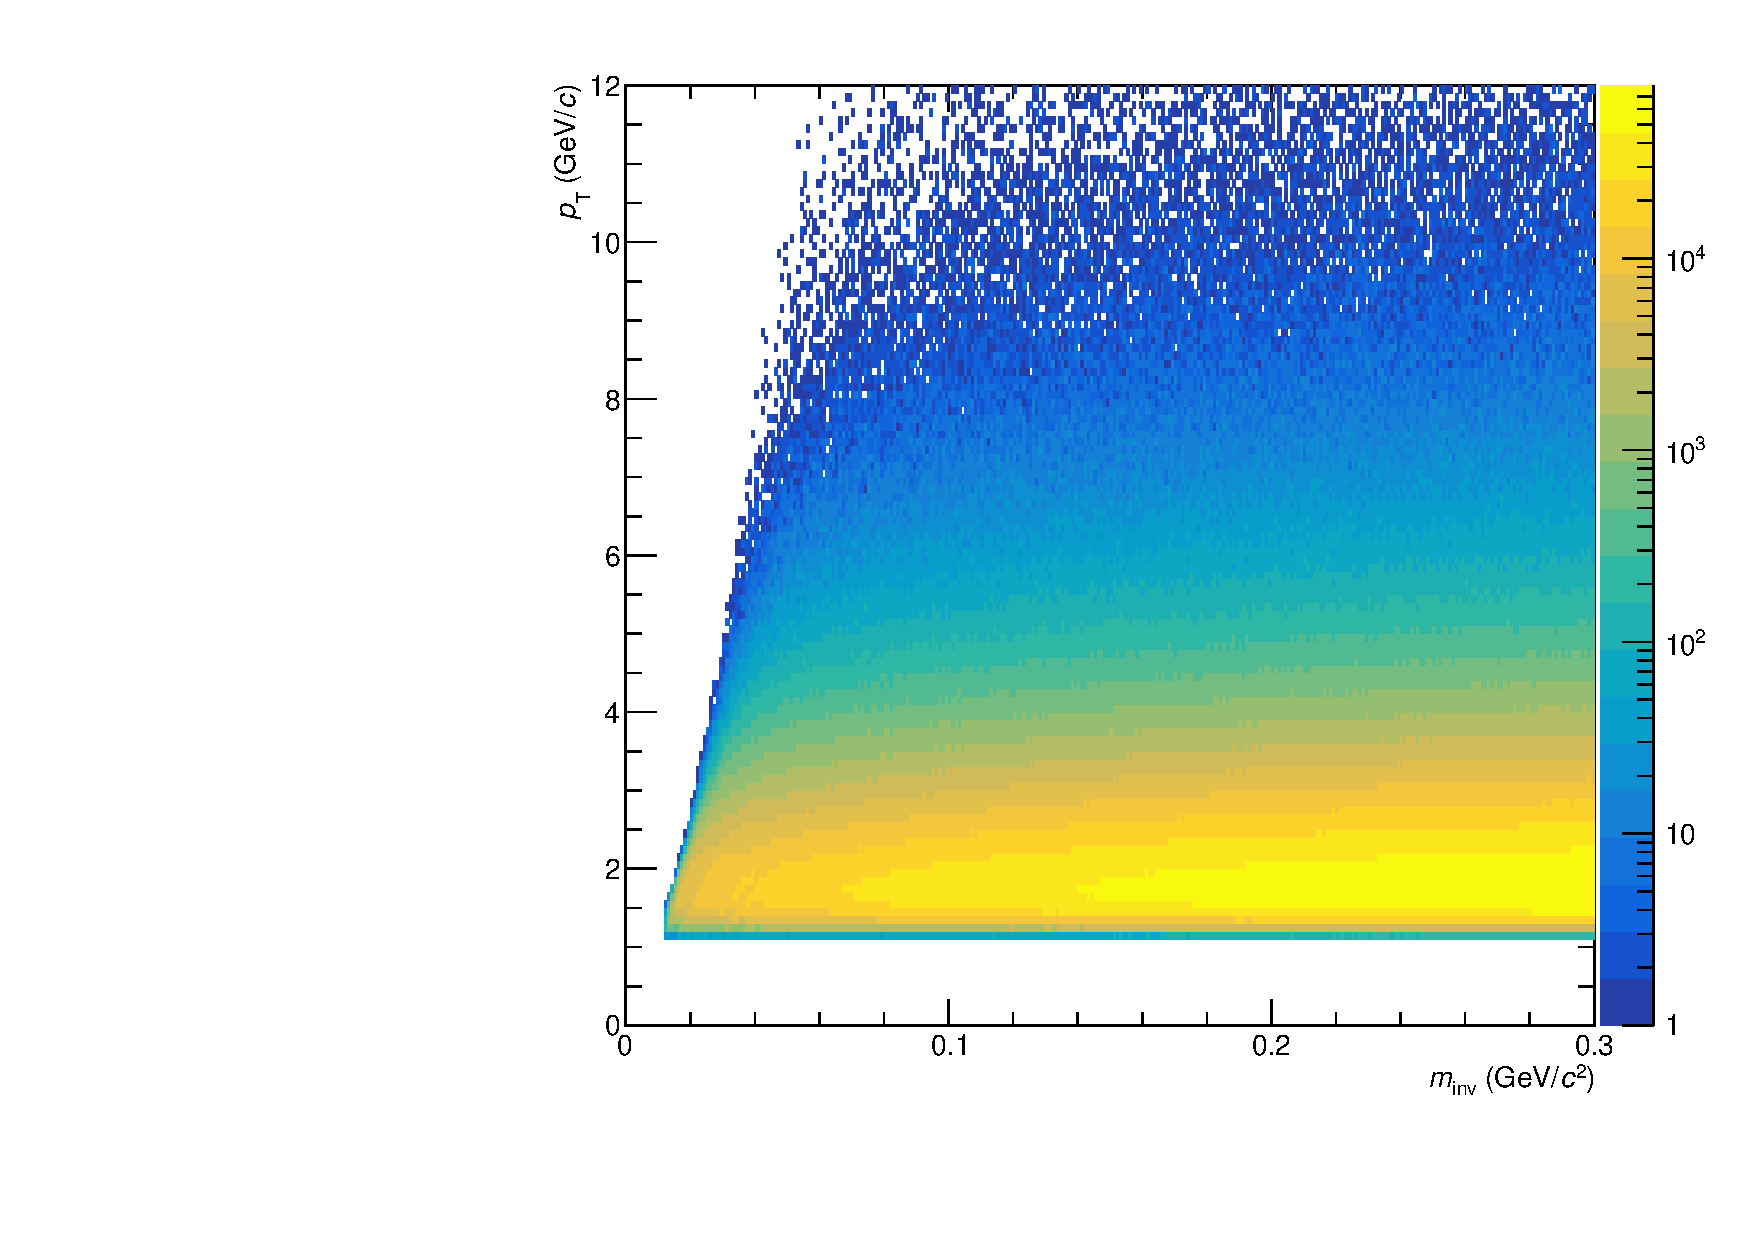
\includegraphics[width=.7\linewidth]{hInvMass_pT_Bkg.pdf}
\caption{$p_\text{T}$ und $m_\text{inv}$ als Funktion von der Anzahl von kombinierten  \textit{Clusterpaaren} aus unterschiedlichen \textit{Events}.}
\label{figInvMassPt_b}
\end{figure}
Durch die paarweise Kombinationen aller \textit{Cluster} eines \textit{Events}, wie es in Abschnitt \ref{s3s2} vorgestellt wurde, ensteht unkorrelierter Untergrund.
Um den unkorrelierten Untergrund abzuschätzen werden \textit{Cluster} aus unterschiedlichen \textit{Events} paarweise miteinander kombiniert.
Dadurch wird sichergestellt, dass zwischen den Teilchen, die den \textit{Clustern} zugrunde liegen, keine Korrelation besteht, sie also unkorreliert sind.
Diese Methode wird als \textit{mixed Event} Methode bezeichnet.
Abbildung \ref{figInvMassPt_b} zeigt die Anzahl \textit{Clusterpaare} als Funktion von $p_\text{T}$ und $m_\text{inv}$, bei der \textit{Cluster} aus unterschiedlichen \textit{Events} miteinander kombiniert wurden.
Da keine Korrelationen zwischen den \textit{Clustern} vorliegen, gibt es keine Häufung der Datenpunkte um eine bestimmte invariante Masse.
\newline
Im selben \textit{Event} würden \textit{Cluster}, die näher als eine Zelldiagonale aneinander liegen mit großer Wahrscheinlichkeit zu einem \textit{Cluster} zusammengefasst werden.
Beim Kombinieren von \textit{Clustern} aus unterschiedlichen \textit{Events} wird der Abstand von zwei \textit{Clustern} durch die Anforderung an den Öffnungswinkel auf mindestens eine Zelldiagonale gesetzt.
Durch diese Anforderung gibt es, wie zuvor in Abschnitt \ref{s3s2} Abbildung \ref{figInvMassPt_a}, eine $p_\text{T}$ abhängige untere Grenze für $m_\text{inv}$.
\newline
In der \textit{mixed Event} Methode gibt es eine größere Anzahl an Kombinationsmöglichkeiten, als in der \textit{same Event} Methode.
Daraus resultiert eine größere Anzahl an Einträgen in der Verteilung der invarianten Masse und des Transversalimpulses aus der \textit{mixed Event} Methode, als in der Verteilung aus der \textit{same Event} Methode.
Deshalb muss die Verteilung, die aus der \textit{mixed Event} Methode kommt, skaliert werden.
Die Skalierung erfolgt bei $m_\text{inv} \in \left[0\,19,3\,0\right] (\text{GeV/}c^{2})$, da dort kein Signal erwartet wird.
Es ergibt sich für den Skalierungsfaktor:
\begin{align}
\label{eqBackSkalierung}
\alpha &= \frac{\sum_{i \neq j}\sum_{n}m_{\text{inv}}\left( \gamma^{(n)}_{i},\gamma^{(n)}_{j}\right) }{\sum_{i,j}\sum_{n \neq m}m_{\text{inv}}\left( \gamma^{(n)}_{i},\gamma^{(m)}_{j}\right) }
\end{align}
Die oberen Indizes $m$ und $n$ stehen hierbei für ein Event, aus dem ein Photon kommt, und die unteren Indizes $i$ und $j$ nummerieren die Photonen ($\gamma$).
\begin{figure}[tp]
\centering
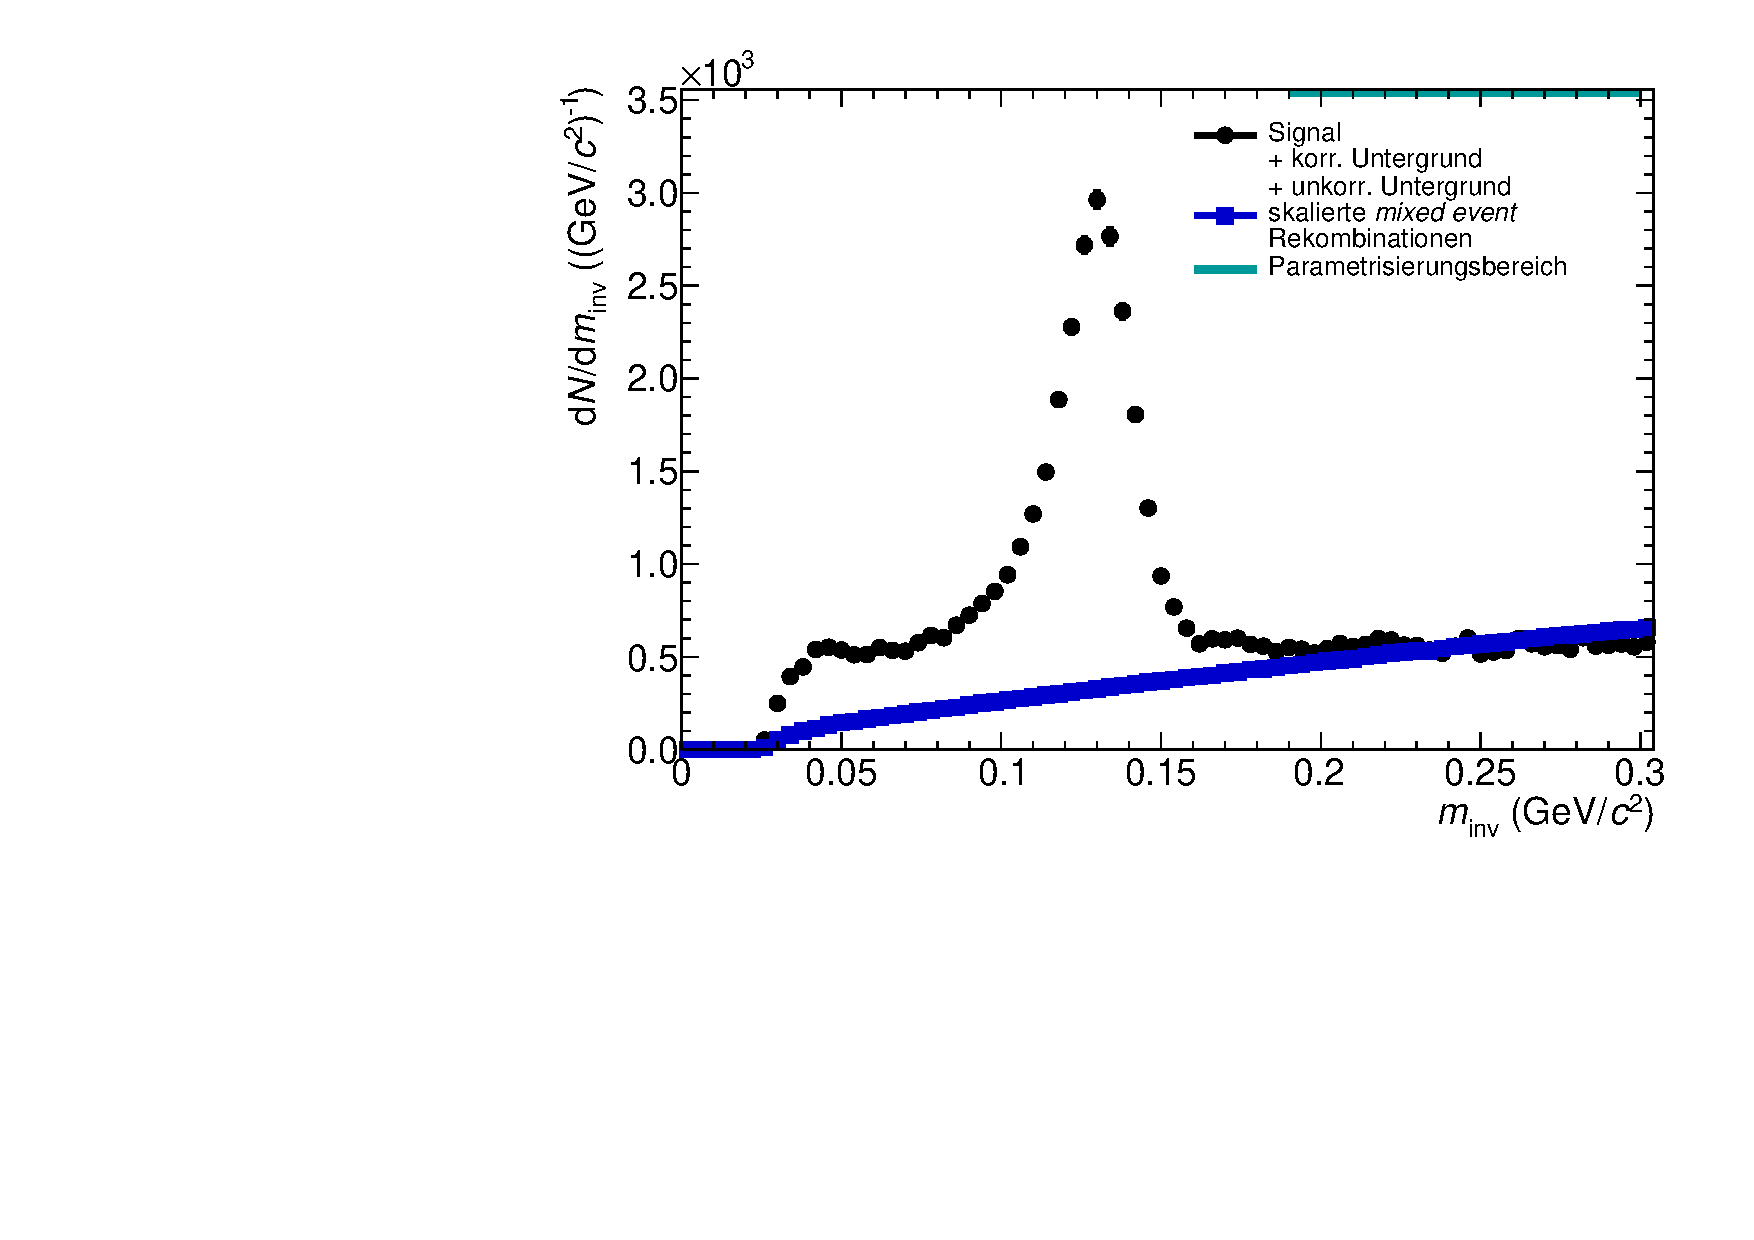
\includegraphics[width=.75\linewidth]{hUncorrBkgNorm.pdf}
\caption{Nach Gleichung \ref{eqBackSkalierung} skalierte {\it mixed Event} Kombinationen als Abschätzung des unkorrelierten Untergrunds zusammen aufgetragen mit Signal zuzüglich beider Untergrundkomponenten wie in Abbildung \ref{figSignalPlusBkg}.}
\label{figUncorrBkgNorm}
\end{figure}
\newline
Abbildung \ref{figUncorrBkgNorm} zeigt die skalierten \textit{mixed Event} Kombinationen und die \textit{same Event} Kombinationen.
Der unkorrelierten Untergrund wird mit steigendem $m_\text{inv}$ größer und macht den Großteil der Anzahl an Einträge für $m_\text{inv} > 0,2 \text{ GeV/}c^{2}$ in der Verteilung der invarianten Masse aus. 
Nachdem der unkorrelierte Untergrund abgeschätzt worden ist, wird dieser von der Verteilung der invarianten Masse aus der \textit{same Event} Methode abgezogen.
\begin{figure}[tp]
\centering
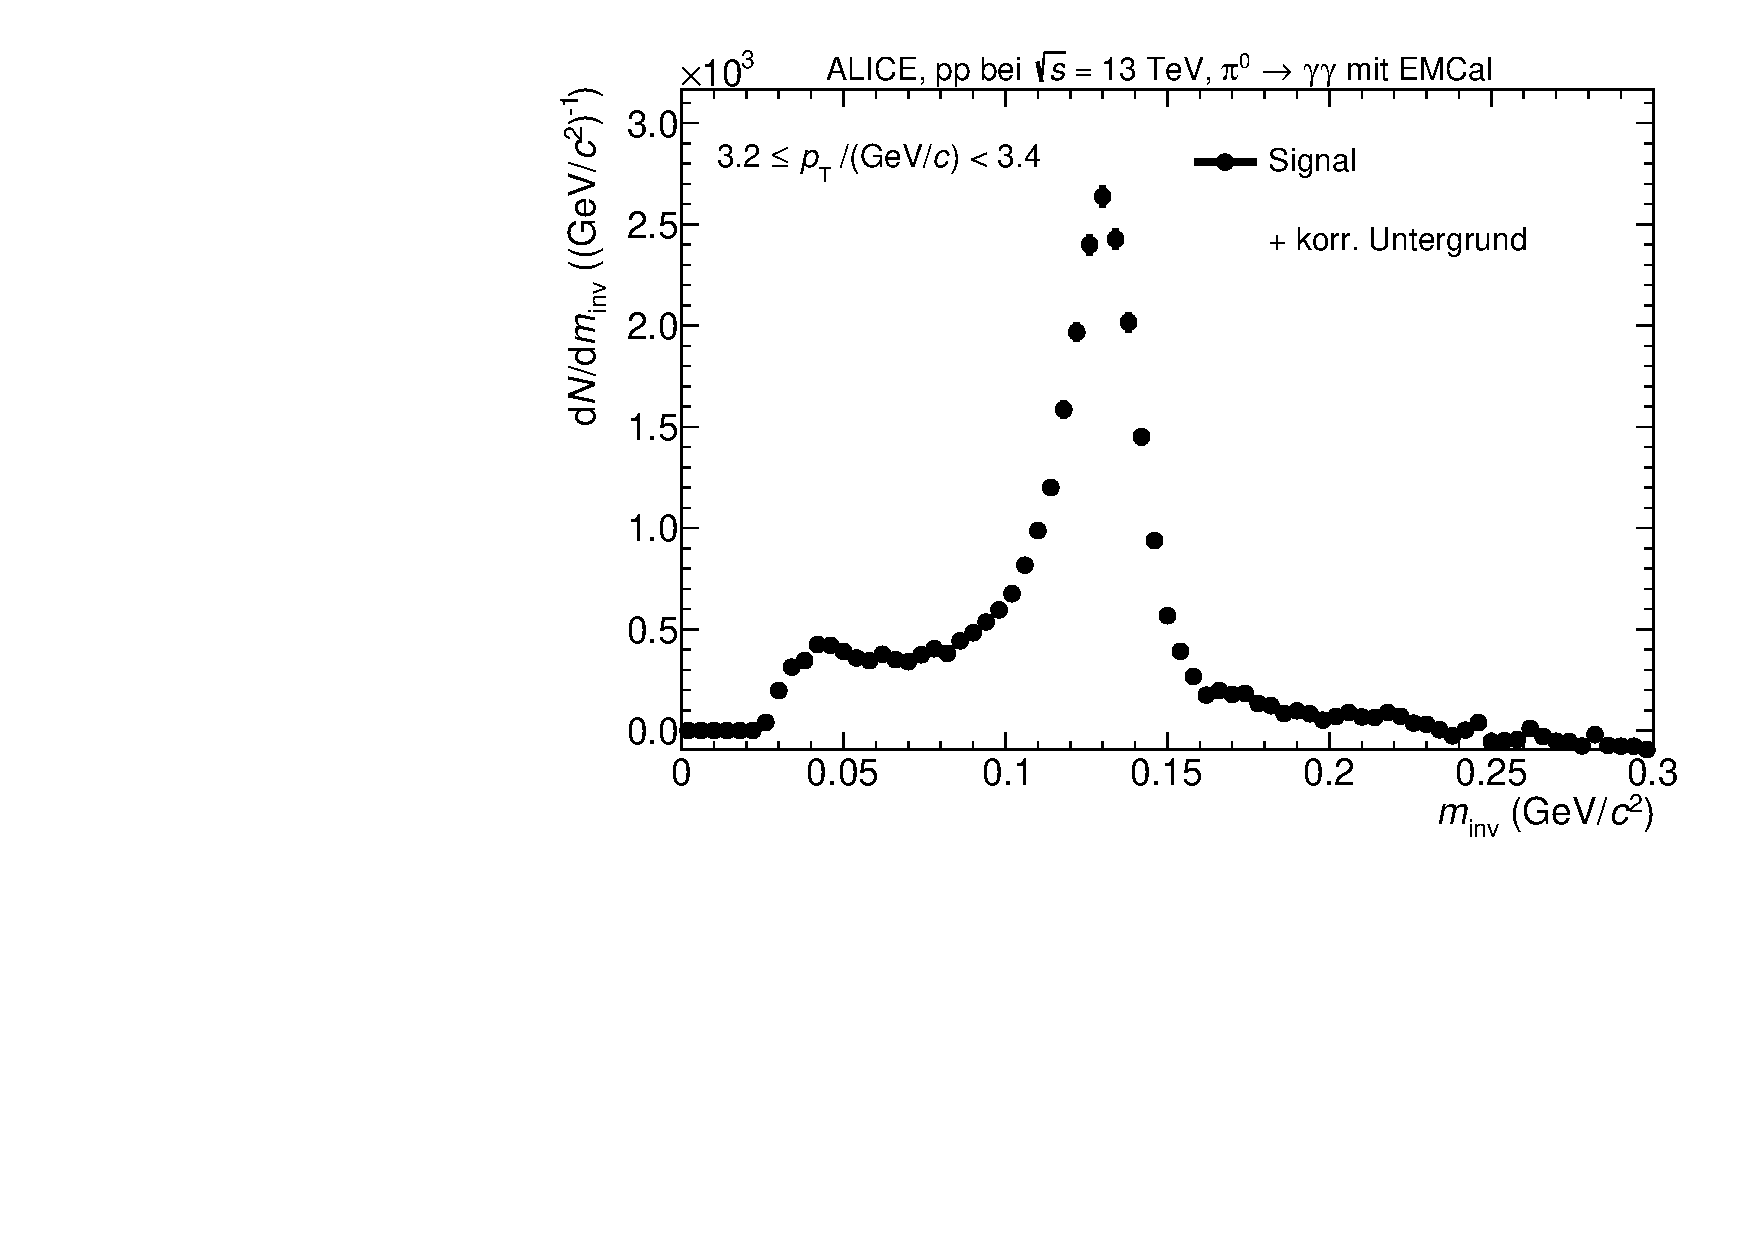
\includegraphics[width=.75\linewidth]{hInvMass_Data.pdf}
\caption{Verteilung der invarianten Masse aus der \textit{same Event} Methode nach Abzug des unkorrelierten Untergrunds.}
\label{figInvMass_Data}
\end{figure}
\newline
Abbildung \ref{figInvMass_Data} zeigt die Verteilung der invarianten Masse aus der \textit{same Event} Methode in dem $p_\text{T}$-Intervall von $(3,2 - 3,4) (\text{GeV/}c)$, nachdem die skalierte Verteilung aus der \textit{mixed Event} Methode abgezogen wurden.
\newline
Der nächste Schritt in der Analyse neutraler Pionen ist die Bestimmung des korrelierten Untergrunds.
Das Abschätzen mit einer linearen Funktion hat sich als gängigste Methode zur Abschätzung des korrelierten Untergrunds entwickelt und wird im Folgenden als Standardmethode bezeichnet.
In dieser Arbeit wird der korrelierte Untergrund sowie das $\pi^{0}$-Signal mit Hilfe von Monte Carlo Templates bestimmt.
Die Ergebnisse der Analyse mit Hilfe von Monte Carlo Templates sowie mit der Standardmethode werden miteinander vergleichen, um eine Aussage über den möglichen Nutzen der Verwendung von Monte Carlo Templates in der Analyse von $\pi^{0}$ treffen zu können.
Im folgenden Abschnitt wird zunächst die Standardmethode kurz erläutert.
